\documentclass[a4paper, 11pt]{report}
\usepackage{cs_thesis}
\usepackage[pdftex]{graphicx}
\usepackage[utf8]{inputenc}
\usepackage{amsmath}
\usepackage{url}
\usepackage{biblatex}
\usepackage{dtklogos}
\usepackage{listings}
\usepackage{color}
\usepackage[tocflat]{tocstyle}
\usetocstyle{standard}

\usepackage{blindtext}
\makeatletter
\renewcommand\tableofcontents{
\hfill\textbf{\Large\contentsname}\hfill\null\par
\@mkboth{\MakeUppercase\contentsname}{\MakeUppercase\contentsname}%
\@starttoc{toc}
}
\makeatother

\renewcommand{\UrlFont}{\small\tt}
\makeatletter
\def\footnoterule{\kern-8\p@
\hrule \@height 1pt \@width 6in \kern 7.6\p@}
\renewcommand{\thempfootnote}{\arabic{mpfootnote}}
\makeatother

\lstset{language=C++,
basicstyle=\ttfamily,
keywordstyle=\color{blue}\ttfamily,
stringstyle=\color{red}\ttfamily,
commentstyle=\color{green}\ttfamily,
morecomment=[l][\color{magenta}]{\#}
}

\lstset{language=C++,
keywordstyle=\color{blue},
stringstyle=\color{red},
commentstyle=\color{green},
morecomment=[l][\color{magenta}]{\#}
}

\title{The iCub Humanoid Robot}
\author{Semih Onay}
\program{Computer Science}
\supervisor{Associated Professor Elena Battini Sönmez}


\begin{document}
\pagenumbering{arabic}
\makecstitle
\tableofcontents
\listoffigures

\begin{symabbreviations}
  \sym{YARP}{Yet Another Robot Platform}
  \sym{ACE}{The ADAPTIVE Communication Environment} 
  \sym{ODE}{Open Dynamics Library}
  \sym{OpenGL}{Open Graphics Library}
  \sym{SDL}{Simple DirectMedia Layer}
\end{symabbreviations}
\chapter{ABSTRACT}
Intelligent agents with human level of proficiency is the ultimate challenge 
for science and technology. Especially for the artificial intelligence field. 
Desing of such systems now eager to evolve and behave like humans. 
Recent discoveries in this field are focused on training  communication 
skills with perception, classification and action which are modelled from 
humans. They are systems that are capable of recieving environmental 
activities(stimulus) and communication. This paper presents a cognitive 
humanoid robot that combines abilities such as object detection, image 
aqusition, language and movement. Aim is to understand how motor control 
abilities, visio-motor abilities and linguistics are designed and developed. 
Study includes robotic simulation applications. Cognitive modules will be 
developed by using application templates and documentation.
\linebreak
{Keywords} : cognitive science,humanoid robots,iCub
\chapter{INTRODUCTION}
The iCub is a humanoid robot that developed at Istituto Italiano di 
Tecnologia (IIT) as part of European project RobotCub and later adopted by 
more 
than 20 laboratories arround the world. It has 53 motors that can move the 
head, arms and hands, midriff, and legs.It can see and hear, it has the sense 
of proprioception\footnote{Body configuration and movement using accelerometers 
and gyroscopes}. It’s designed to aid studies of human cognition and artificial 
intelligence. Project members developed computer simulator to experiment new 
techniques.\par 
Computer simulations are getting important in area robotics area.Simulations 
may not provide real complexity of the physical world and 
not reliable as real dynamics. The simulator of iCub is an easy way to test 
new algorithms and methods instead of dealing with complex configuration of 
iCub hardware. The simulator is designed to be accurate as real world 
psychics and dynamics. Development is based on directly from first prototype 
of simulation environment Webots.\footnote{Webots : 
  https://www.cyberbotics.com}It was 
expensive and had limited access to source code which made hard to modify 
source code in order to add some functionalties.Then iCub simulation created. 
Simulation environment uses \linebreak to simulate body 
movement and collision detection algorithms to measure psychical interaction 
with the world. ODE\footnote{Open Dynamics Engine : http://www.ode.org} is 
used in wide range of projects like GAZEBO\footnote{GAZEBO : 
  http://gazebosim.org}. ODE is an open source physics engine forauthoring 
  tools, 
computer games,etc.It uses OpenGL\footnote{Open Graphics Library : 
  https://www.opengl.org} renderer and it has some disadvantages due to 
limitation of OpenGL engine computation efficiency on complex structures. 
iCub 
simulation is using OpenGL directly via SDL\footnote{Simple DirectMedia Layer 
: 
  https://www.libsdl.org}which helps to render complex robot movements and 
computationally efficient simulation observations. The aim of this study is to 
experiment and understand how cognitive architecture of robotics designed and 
implemented. 

{\tiny}\chapter{LITERATURE REVIEW}
Development of simulator is described by abstraction of parts to handle 
complex instructions more precisely and efficient. Some other external 
software 
libraries are used to reduce required time to animate given parts of robots 
body from parameters. Abstractions made it easy to implement new 
methods,algorithms into a simulation environment. Understanding of these 
libraries are the key of creating new interfaces and methods to robot in 
virtual world. Action primitives are pre-defined inside a simulation 
environment to extendcapability of creating new interfaces to virtual 
simulation world and can be changed or taught as different languages which 
helps to extend knowledge about languages.


The great challenges in robotics is to imitate human behaviour. Most of the 
humanoid robots have some perception to recognize their surroundings 
autonomosly. Grasping an object in its environment, is one of the most 
difficult tasks for all kinds of robots. Many parameters must be provided for, 
the objects, surroundings, and the specification of the assignment. Taking 
these parameters into consideration, the ability to receive sensing information 
from the robot is crucial when implementing an efficient robotic grasp. The 
quality of the sensing information 
must also be taken into consideration, as signals may limit precision and can 
potentially be noisy. In recent years, there have been several models 
implemented to perform a grasping behavior.\cite{V. Tikhanoff, A. Cangelosi, G. 
Metta  Platform}


\begin{itemize}
\item Knowledge based grasp action,
\item Geometric grasp action,
\item Sensor driven and learning based grasping.
\end{itemize}
\chapter{METHODOLOGY}
\subsection{The iCub Cognitive Architecture}
The architecture consists of modules and sub-modules. Their relations are 
similar to the human mental system. Gaze controling, reaching, and locomotion 
establishes the simple goal oriented actions. Episodic and procedural memories 
are effects a simple version of an internal simulation to provide capabilities 
for prediction and reconstruction, as well as productive model construction 
by experienced affordances from environmental sensors. A simple process of 
homeostatic state is achived by the affective state that provides action 
selection and attention selection. These futures are already implemented in the 
simulation environment.
\begin{figure}[h!]
  \centering
  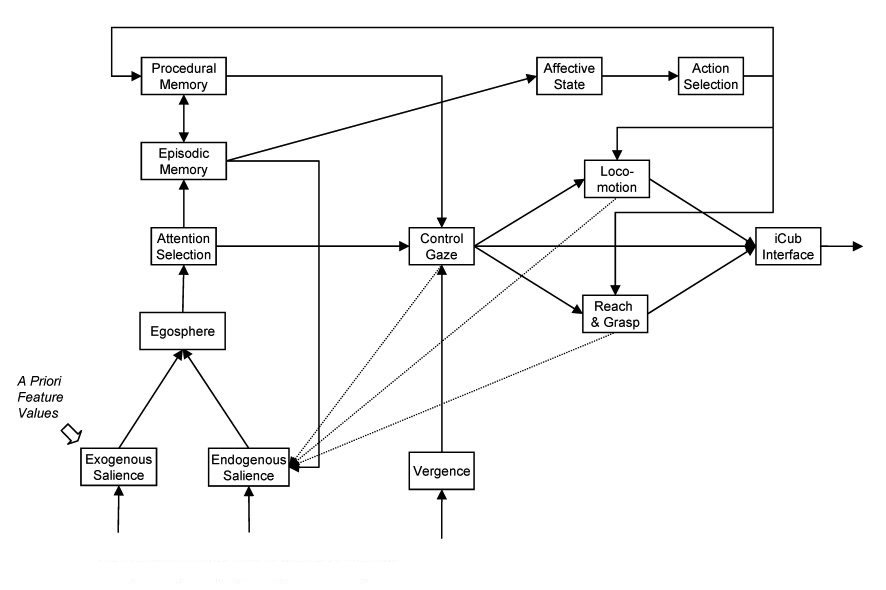
\includegraphics[width=1.0\linewidth]{cognitive_architecture}
  \caption{General View of iCub Cognitive Architecture}
  \label{fig:cognitive_architecture}
 \end{figure}
Indiviual components of the architecture operates synchronously for a series of 
states representing cognitive behaviour that emerges from the interaction of 
separate parallel processes instead of being governed by some state machine as 
it like the most of cognitive architectures. In addition, motivations are 
encapsulated in the affective state of the system. They are designed explicitly 
to address curiosity and experimentation by using explorative motives which are 
triggered by exogenous and endogenous factors, respectively. Distinction 
between the exogenous and endogenous salience is represented by the need to 
include an attention system to consolidate both factors.
\newpage
\subsection{The Embodiment}
It is developed as an embodied agent by its physical components joints, 
actuators, and a many of sensors that are providing internal stimuli and 
external stimuli information about the body and its surroundings. 
Actuation is effected through a variety of DC motors and servo-motors. Sensory 
data provides joint position, velocity of movements, and torque, streamed video 
images from the head eye cameras, audio from the left and right ear 
microphones\cite{David Vernon}. Accessing to the motor control and sensor 
interface is provided through iCubInterface in the cognitive architecture in 
Fig. 5.1 This module is represented as an YARP software module iCubInterface.
That interface turns relevant data into actions.
\subsection{Software Representation}
Software implementation is shown in Figure 5.2 has been realized as a complete 
software system consist of a YARP and iCub modules. All modules are connected 
internally and communicates through YARP ports and they can be called from a 
application or from command line interface with required paramaters. These 
modules are:
\begin{itemize}
  \item salience
  \item endogenousSalience
  \item egoSphere
  \item attentionSelection
  \item episodicMemory
  \item proceduralMemory
  \item affectiveState
  \item actionSelection
  \item controlGaze2
  \item logPolarTransform
  \item cameraCalib
\end{itemize}
\begin{figure}[h!]
  \centering
  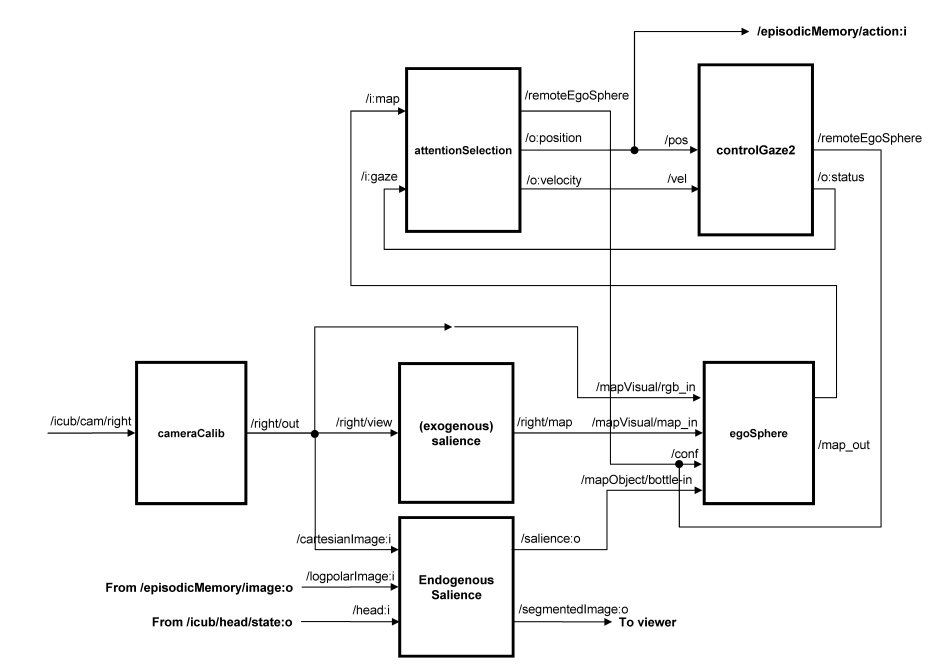
\includegraphics[width=0.8\linewidth]{cognitive_architecture_A}
  \caption{iCub Internal Architecture}
  \label{fig:cognitive_architecture_A}
\end{figure} 
\newpage
\subsection{The YARP}
It is a set of open source libraries that supports modularity by 
using abstraction method in softwares to handle common difficulties in 
robotics area which are know as modularity algorithms, hardware interfaces and 
OS platforms.To deal with OS spesific builds,requires to use cross-platform 
build tools such as CMake\footnote{CMake : http://www.cmake.org} and 
ACE\footnote{The ADAPTIVE Communication Environment :
  http://www.cs.wustl.edu/~schmidt/ACE.html}. YARP is providing platform 
independence. First abstraction can be described as a protocols. Main YARP 
protocol manages interprocess communications in operating systems. It can 
deliver process messages of any size across the network by using different 
protocols.
\begin{figure}[h!]
  \centering
  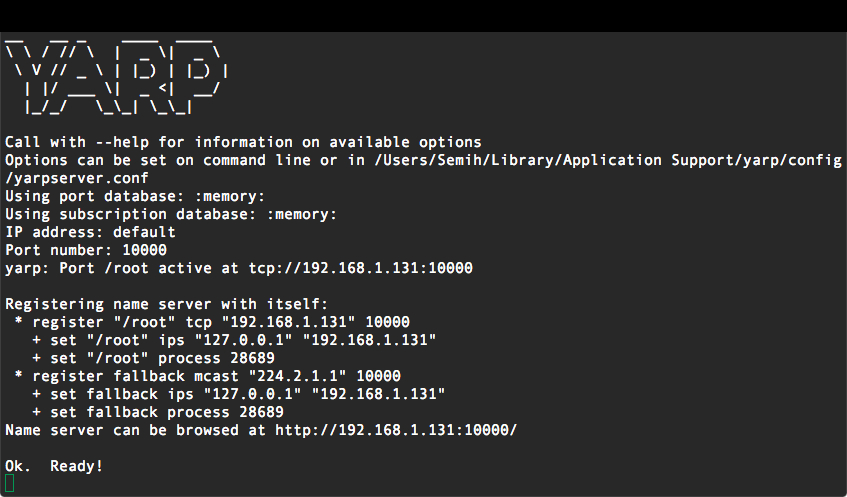
\includegraphics[width=1.0\linewidth]{yarp}
  \caption{YARP Command Line Interface}
  \label{fig:yarp}
\end{figure}
Second abstraction is about hardware communications.The method is to define 
interface for class of devices to fold native coded APIs.Changes in hardwares 
requires changes in API\footnote{API : Application Programming Interface} calls 
via linking suitable libraries to encapsulate 
hardware dependency problems. These abstractions combined to use remote 
device drives where that can be accessed across the network like a parallel 
processing.
The purpose of YARP ports are to move data from threads to threads over the 
processes.Flow of the data can be configured and observed from command-line 
at real time. Port can receive or send data from any other port.Connections 
between ports can be modified easily with using different protocols such as 
TCP\footnote{Transmission Control Protocol} and UDP\footnote{UDP : User 
Datagram Protocol}.The choice depends on quality of message transmission or 
response 
time. Using TCP is for reliability and UDP is for speed with effect on 
unreliable transmissions. As it seen in Figure 5.3 it registers a name server 
over localhost and assigns root node to branching iCub components.
\newpage
\subsection{iCub Simulation Environment}
The computer simulation model of the iCub allows to create realistic scenarios 
in where robot can interact with a virtual world and physical limitations, 
interactions that occur between the virtual world is simulated using open 
source library ODE to provide accurate simulation of body dynamics.
Simulation surroundings can be manipulated by a single configuration file which 
contains ; textures, objects, default arm positions, video configurations and 
calibration settings. In order to place some objects in the environment, it 
needs to be spawned by using the command line interface. Environment supports 
direct frame streaming through yarpview application.
\begin{figure}[h!]
\centering
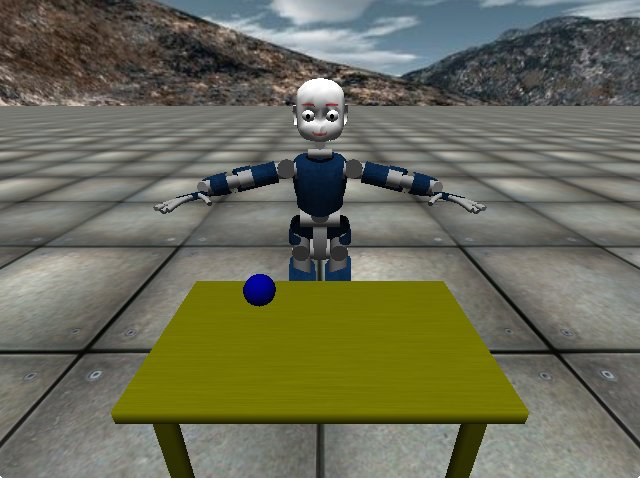
\includegraphics[width=0.5\linewidth]{sim}
\caption{iCub Simulation Environment}
\label{fig:icub}
\end{figure}
\chapter{CONCULUSIONS}
\subsection{Speech Synthesis}
Speech module has ability to speak given text inputs only in English language. 
A new Module developed from application template with open source text to 
speech library. iCub now can speak Turkish language. Module can be extended to 
synthesis of another languages. eSpeak wrapper can provide various of language 
sound database. Speech Recognition module exists but it needs some Windows 
system libraries.
\subsection{Object Grasping}
Module tested with example data sets. It can grasp an object from table. It 
requires that other modules support. Required modules must be running before 
the grasping module. It needs to be trained from a neural network file.
\subsection{Image Capture}
An application developed from templates to capture actual action sequences from 
head camera. Images can be streamed as a video.
\subsection{Sound I/O}
Small module developed to send sound commands from computer microphone. Module 
documentation was not enough descriptive to create new audio ports for speech 
recognition. Some applications were not complied at all.
\par 
All implementations are avaible on \bf GitHub.


\appendix
\chapter{Sample Code Snippets}
\subsection{Turkish Synthesis Module}
\begin{lstlisting}
class iSpeak : protected BufferedPort<Bottle>,
public    RateThread
{
string name;
string package;
string package_options;
deque<Bottle> buffer;
Mutex mutex;

bool speaking;
MouthHandler mouth;

// gets text sequence
void speak(const string &phrase)
{
string command("echo \"");
command+=phrase;
command+="\" | ";
command+=package;
command+=" ";

// Check for speech synthesis library
if (package=="espeak")
command+="-v turkish --stdin";

// Get text input from CLI
command+=package_options;
//int ret=system(command.c_str());
}

void run()
{
string phrase;
double time;
bool onlyMouth=false;
int rate=(int)mouth.getRate();
bool resetRate=false;
double duration=-1.0;

mutex.lock();
// protecting also the access of size() function
if (buffer.size()>0)    
{
// allocate space from yarp Bottle
Bottle request=buffer.front();
buffer.pop_front();

if (request.size()>0)
{
if (request.get(0).isString())
{
phrase=request.get(0).asString().c_str();
speaking=true;
}
else if (request.get(0).isDouble() || request.get(0).isInt())
{
time=request.get(0).asDouble();
speaking=true;
onlyMouth=true;
}

}
\end{lstlisting}
\subsection{Object Mover Module}
\begin{lstlisting}
public:objectMoverThread(ResourceFinder &_rf) : rf(_rf) {
virtual bool loadParams() {
name = rf.check("name",Value("objectMover")).asString().c_str();
neckTT = rf.check("necktt",Value(2.0)).asDouble();
eyeTT = rf.check("eyett",Value(1.2)).asDouble();
trajTime = rf.check("trajtime",Value(4.0),"Solver trajectory 
time").asDouble();
maxPitch = rf.check("maxpitch",Value(30.0),"Torso max pitch").asDouble();

//get which arm to use. default to left if they didnt pass in left or right
armname = rf.check("arm", Value("left"),"arm name").asString().c_str();
if (armname == "right") {
armInUse = true;
}
else {
armInUse = false;
}
//get robot name to use (icubSim is for simulation)
robotname = rf.check("robot", Value("icubSim"),"robot name").asString().c_str();
}
\end{lstlisting}

\appendix

\chapter{Screenshots}
\begin{figure}[h!]
  \centering
  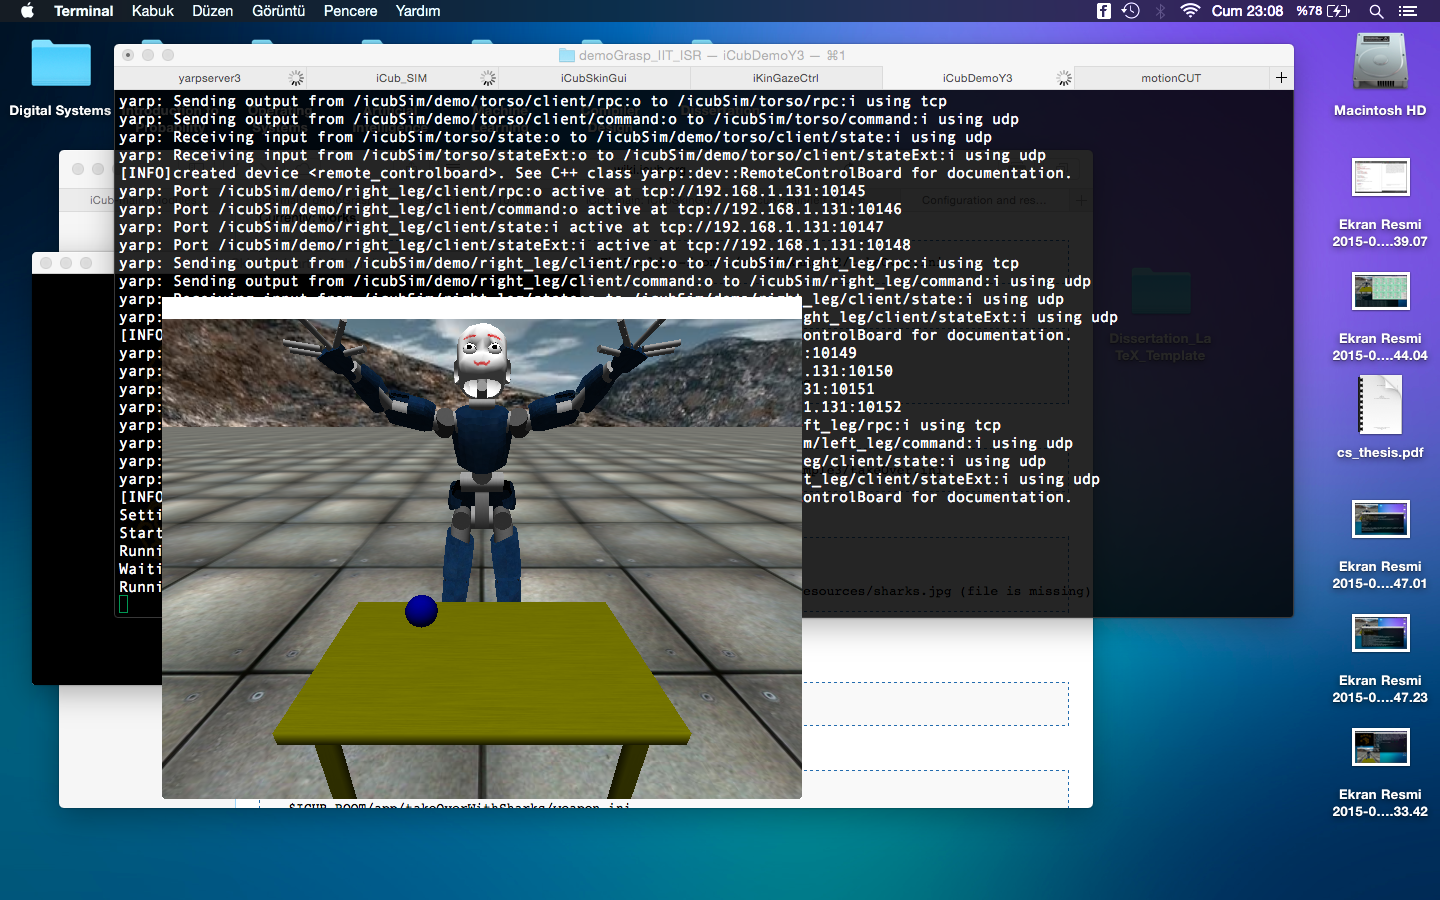
\includegraphics[width=1.0\linewidth]{fullBody}
  \caption{Full Body Movement}
  \label{fig:fullBody}
\end{figure}
\begin{figure}[h!]
\centering
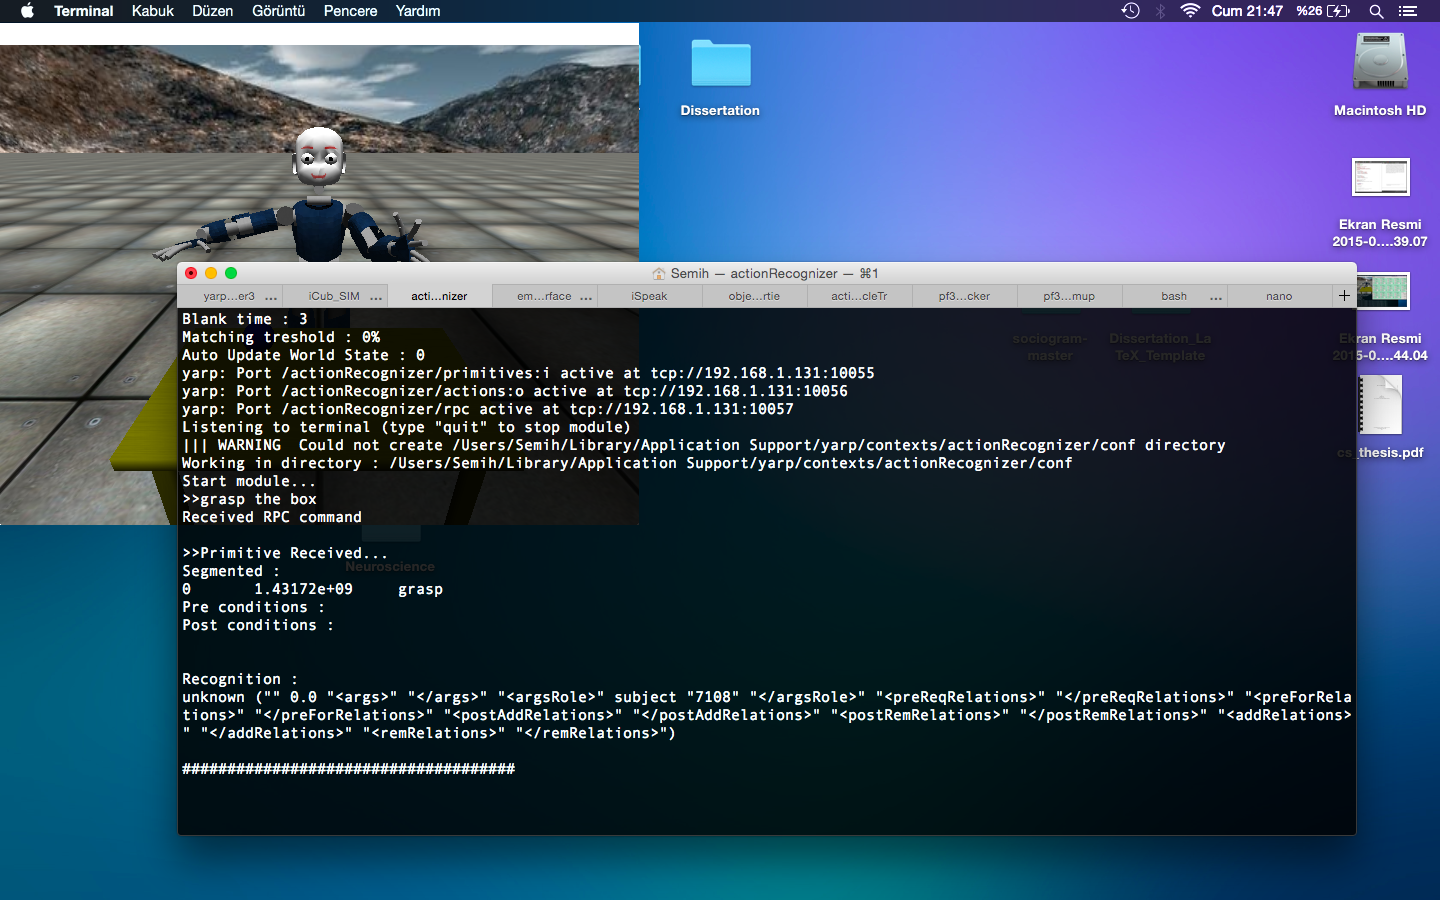
\includegraphics[width=1.0\linewidth]{actionRecognizer}
\caption{Action Recognizer}
\label{fig:actionRecognizer}
\end{figure}
\begin{figure}[h!]
\centering
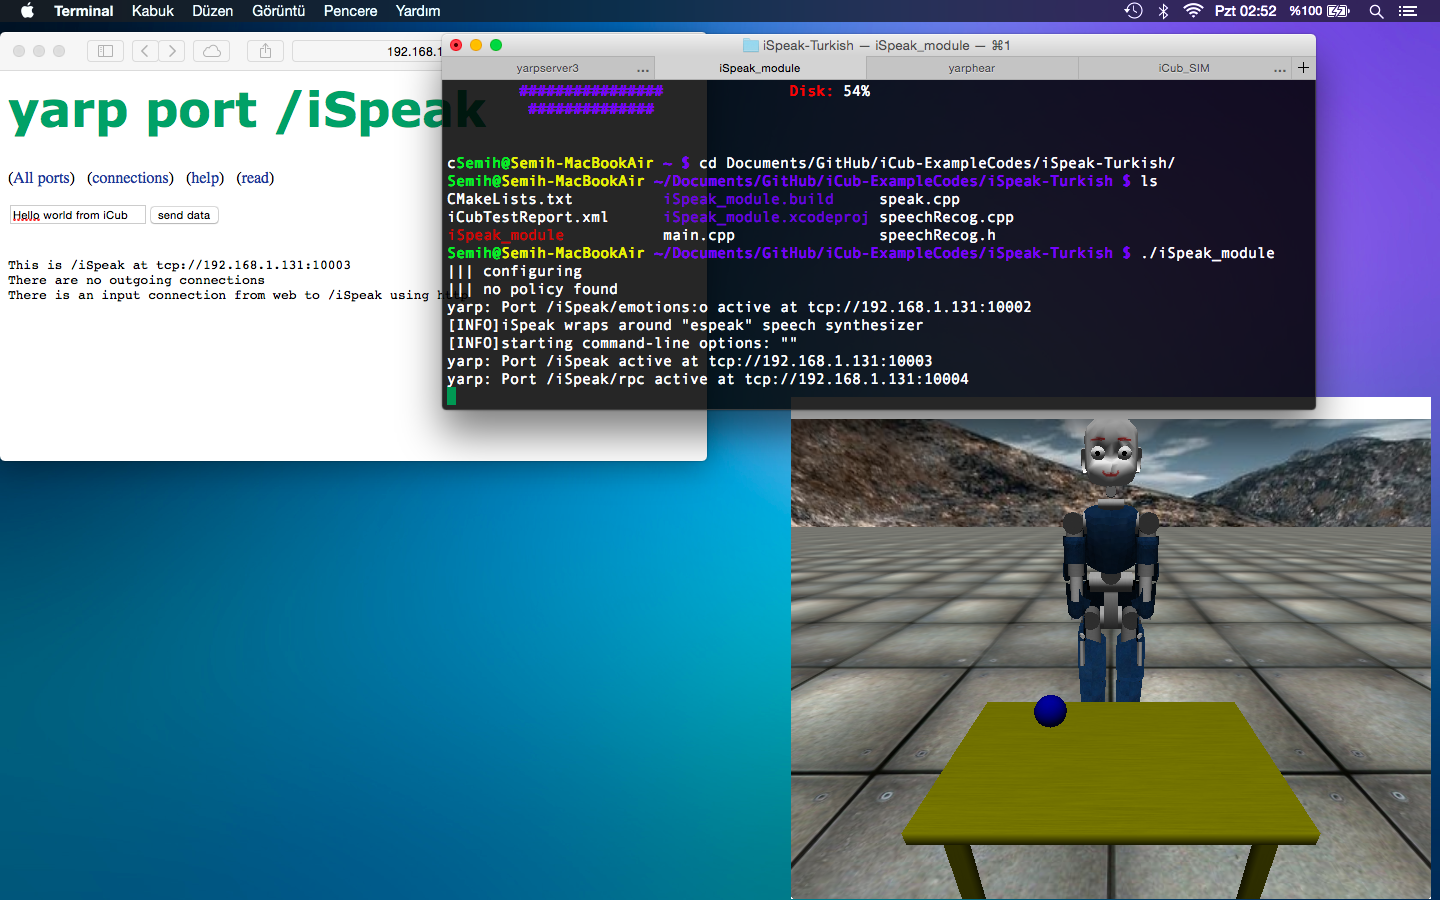
\includegraphics[width=1.0\linewidth]{iSpeak}
\caption{iSpeak Module}
\label{fig:iSpeak}
\end{figure}
\begin{figure}[h!]
\centering
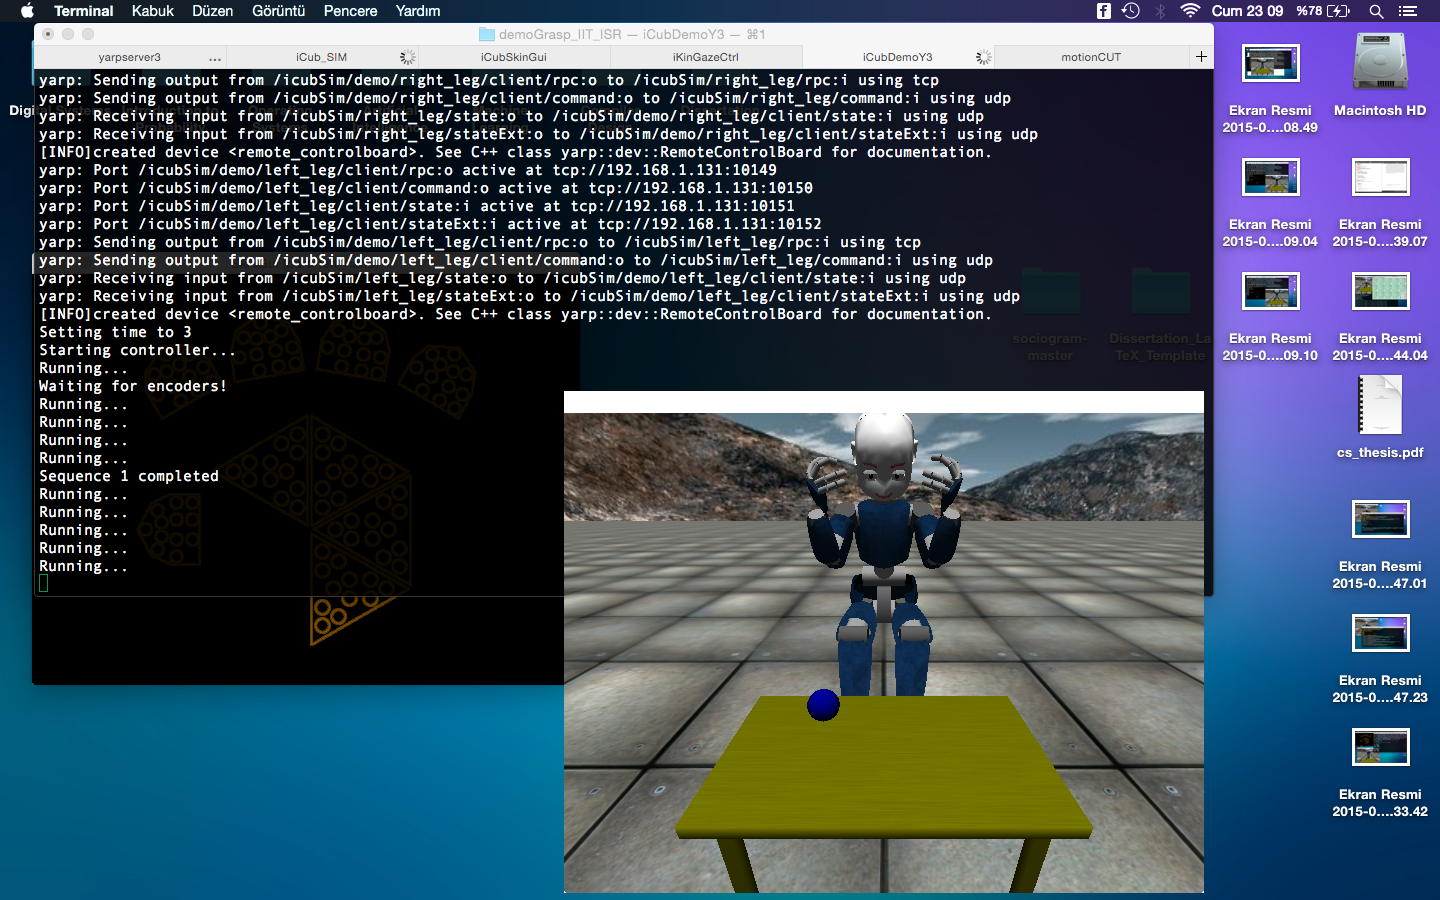
\includegraphics[width=1.0\linewidth]{neural}
\caption{iCub Sample Body Postures}
\label{fig:neural}
\end{figure}


\begin{thebibliography}{9}
  \bibitem{Webots} 
  Webots: Robot simulation software
  \\\texttt{https://www.cyberbotics.com}
  
  \bibitem{ODE} 
  ODE: Open Dynamics Engine
  \\\texttt{http://www.ode.org}
  
  \bibitem{Gazebo}
  Gazebo: Open Source Simulation Environment
  \\\texttt{http://gazebosim.org}
  
  \bibitem{YARP} 
  YARP: Yet Another Robot Platform 
  \\\texttt{http://wiki.icub.org/yarp/}
  
  \bibitem{CMake} 
  CMake: Cross-Platform Open Source Build System 
  \\\texttt{http://www.cmake.org}
  
  \bibitem{ACE} 
  ACE: The ADAPTIVE Communication Environment
  \\\texttt{http://www.cs.wustl.edu/~schmidt/ACE.html}
  
  \bibitem{iCub} 
  iCub: An Open Source Cognitive Humanoid Robotic Platform
  \\\texttt{http://www.icub.org}
  
  \bibitem{David Vernon} David Vernon The iCub [online]. 
  URL 
  \url{http://www.referenceforbusiness.com/biography/A-E/Ballmer-Steve-1956.ht%
    % ml}. Accessed 18 March 2015.
   \bibitem{V. Tikhanoff, A. Cangelosi, G. Metta Platform}
   Speech and Action Integration in Humanoid Robots: Simulation Experiments 
   with iCub, V. Tikhanoff, A. Cangelosi, G. Metta Platform 
  \bibitem{}The iCub humanoid robot: an open platform for research in embodied 
  cognition, Giorgio Metta Giulio Sandini, David Vernon, Lorenzo Natale
Francesco Nori
  \end{thebibliography}
  
\end{document}